

\tikzset{every picture/.style={line width=0.75pt}} %set default line width to 0.75pt        

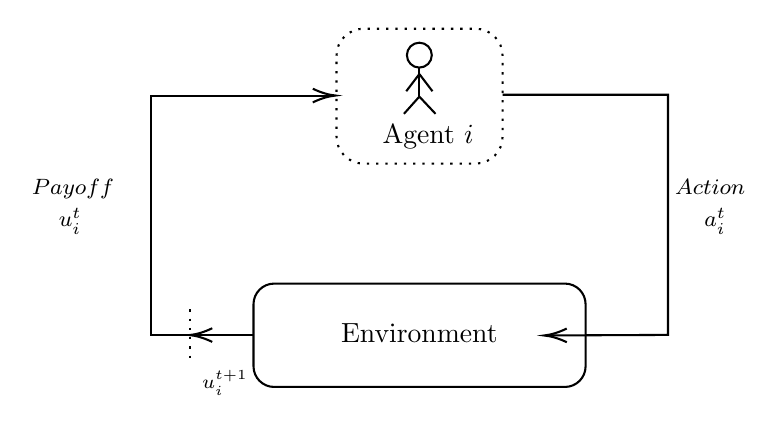
\begin{tikzpicture}[x=0.75pt,y=0.75pt,yscale=-1,xscale=1]
%uncomment if require: \path (0,212); %set diagram left start at 0, and has height of 212

%Rounded Rect [id:dp4614923576655643] 
\draw  [dash pattern={on 0.84pt off 2.51pt}] (280.3,21) .. controls (280.3,13.82) and (286.12,8) .. (293.3,8) -- (347.3,8) .. controls (354.48,8) and (360.3,13.82) .. (360.3,21) -- (360.3,60) .. controls (360.3,67.18) and (354.48,73) .. (347.3,73) -- (293.3,73) .. controls (286.12,73) and (280.3,67.18) .. (280.3,60) -- cycle ;
%Straight Lines [id:da7057839774959118] 
\draw    (360.3,39.8) -- (440.02,39.8) -- (440.02,155.52) -- (382.3,155.79) ;
\draw [shift={(380.3,155.8)}, rotate = 359.73] [color={rgb, 255:red, 0; green, 0; blue, 0 }  ][line width=0.75]    (10.93,-3.29) .. controls (6.95,-1.4) and (3.31,-0.3) .. (0,0) .. controls (3.31,0.3) and (6.95,1.4) .. (10.93,3.29)   ;
%Rounded Rect [id:dp8891418990726014] 
\draw   (240.3,140.76) .. controls (240.3,135.26) and (244.76,130.8) .. (250.26,130.8) -- (390.34,130.8) .. controls (395.84,130.8) and (400.3,135.26) .. (400.3,140.76) -- (400.3,170.64) .. controls (400.3,176.14) and (395.84,180.6) .. (390.34,180.6) -- (250.26,180.6) .. controls (244.76,180.6) and (240.3,176.14) .. (240.3,170.64) -- cycle ;
%Straight Lines [id:da2888293435612861] 
\draw    (209.5,155.6) -- (190.8,155.6) -- (190.8,40.2) -- (277.8,40.2) ;
\draw [shift={(279.8,40.2)}, rotate = 180] [color={rgb, 255:red, 0; green, 0; blue, 0 }  ][line width=0.75]    (10.93,-3.29) .. controls (6.95,-1.4) and (3.31,-0.3) .. (0,0) .. controls (3.31,0.3) and (6.95,1.4) .. (10.93,3.29)   ;
%Straight Lines [id:da2509852546185203] 
\draw    (239.9,155.6) -- (211.5,155.6) ;
\draw [shift={(209.5,155.6)}, rotate = 360] [color={rgb, 255:red, 0; green, 0; blue, 0 }  ][line width=0.75]    (10.93,-3.29) .. controls (6.95,-1.4) and (3.31,-0.3) .. (0,0) .. controls (3.31,0.3) and (6.95,1.4) .. (10.93,3.29)   ;
%Straight Lines [id:da8982963971606834] 
\draw  [dash pattern={on 0.84pt off 2.51pt}]  (209.5,143.2) -- (209.5,169) ;
%Shape: Ellipse [id:dp39240400708385637] 
\draw   (314.21,20.73) .. controls (314.21,17.42) and (316.9,14.74) .. (320.21,14.74) .. controls (323.52,14.74) and (326.2,17.42) .. (326.2,20.73) .. controls (326.2,24.05) and (323.52,26.73) .. (320.21,26.73) .. controls (316.9,26.73) and (314.21,24.05) .. (314.21,20.73) -- cycle ;
%Straight Lines [id:da27031411006830464] 
\draw    (320.21,26.73) -- (320.21,40.97) ;
%Straight Lines [id:da049037716254048735] 
\draw    (320.21,40.71) -- (312.79,49) ;
%Straight Lines [id:da6050526887891938] 
\draw    (320.21,40.71) -- (328,49) ;
%Straight Lines [id:da23739202817698213] 
\draw    (320.21,29.84) -- (313.9,38.12) ;
%Straight Lines [id:da11497148653066769] 
\draw    (320.21,29.84) -- (326.52,38.12) ;

% Text Node
\draw (281,148.64) node [anchor=north west][inner sep=0.75pt]   [align=left] {Environment};
% Text Node
\draw (301,52.64) node [anchor=north west][inner sep=0.75pt]   [align=left] {Agent $i$};
% Text Node
\draw (132,79.2) node [anchor=north west][inner sep=0.75pt]  [font=\footnotesize]  {$Payoff$};
% Text Node
\draw (214,171.2) node [anchor=north west][inner sep=0.75pt]  [font=\scriptsize]  {$u_{i}^{t+1}$};
% Text Node
\draw (145,93.2) node [anchor=north west][inner sep=0.75pt]  [font=\footnotesize]  {$u_{i}^{t}$};
% Text Node
\draw (442,79.2) node [anchor=north west][inner sep=0.75pt]  [font=\footnotesize]  {$Action$};
% Text Node
\draw (456,93.2) node [anchor=north west][inner sep=0.75pt]  [font=\footnotesize]  {$a_{i}^{t}$};


\end{tikzpicture}
